%! Author = Mateusz Budzisz
%! Date = 26/05/2024

\chapter{Realizacja Projektu}
\label{ch:realizacja}
Po zakończeniu prac analitycznych i omówieniu przewidywanych funkcjonalności przeprowadzono analizę możliwych decyzji projektowych. Podjęto działania umożliwiające wybór odpowiednich rozwiązań projektowych. 
Następnie przystąpiono do realizacji poszczególnych komponentów systemu.

\section{Aplikacja City Map Planner}
\label{sec:aplikacja}

\subsection{Przyrost I - utworzenie szkieletu aplikacji oraz Potoki testów aplikacji}
\label{sec:przyrost1}

W ramach tego przyrostu pierwszego wykonano:
\begin{itemize}
    \item backend WebAPI z podstawowym testem działania funkcjonowania;
    \begin{figure}[H]
        \centering
        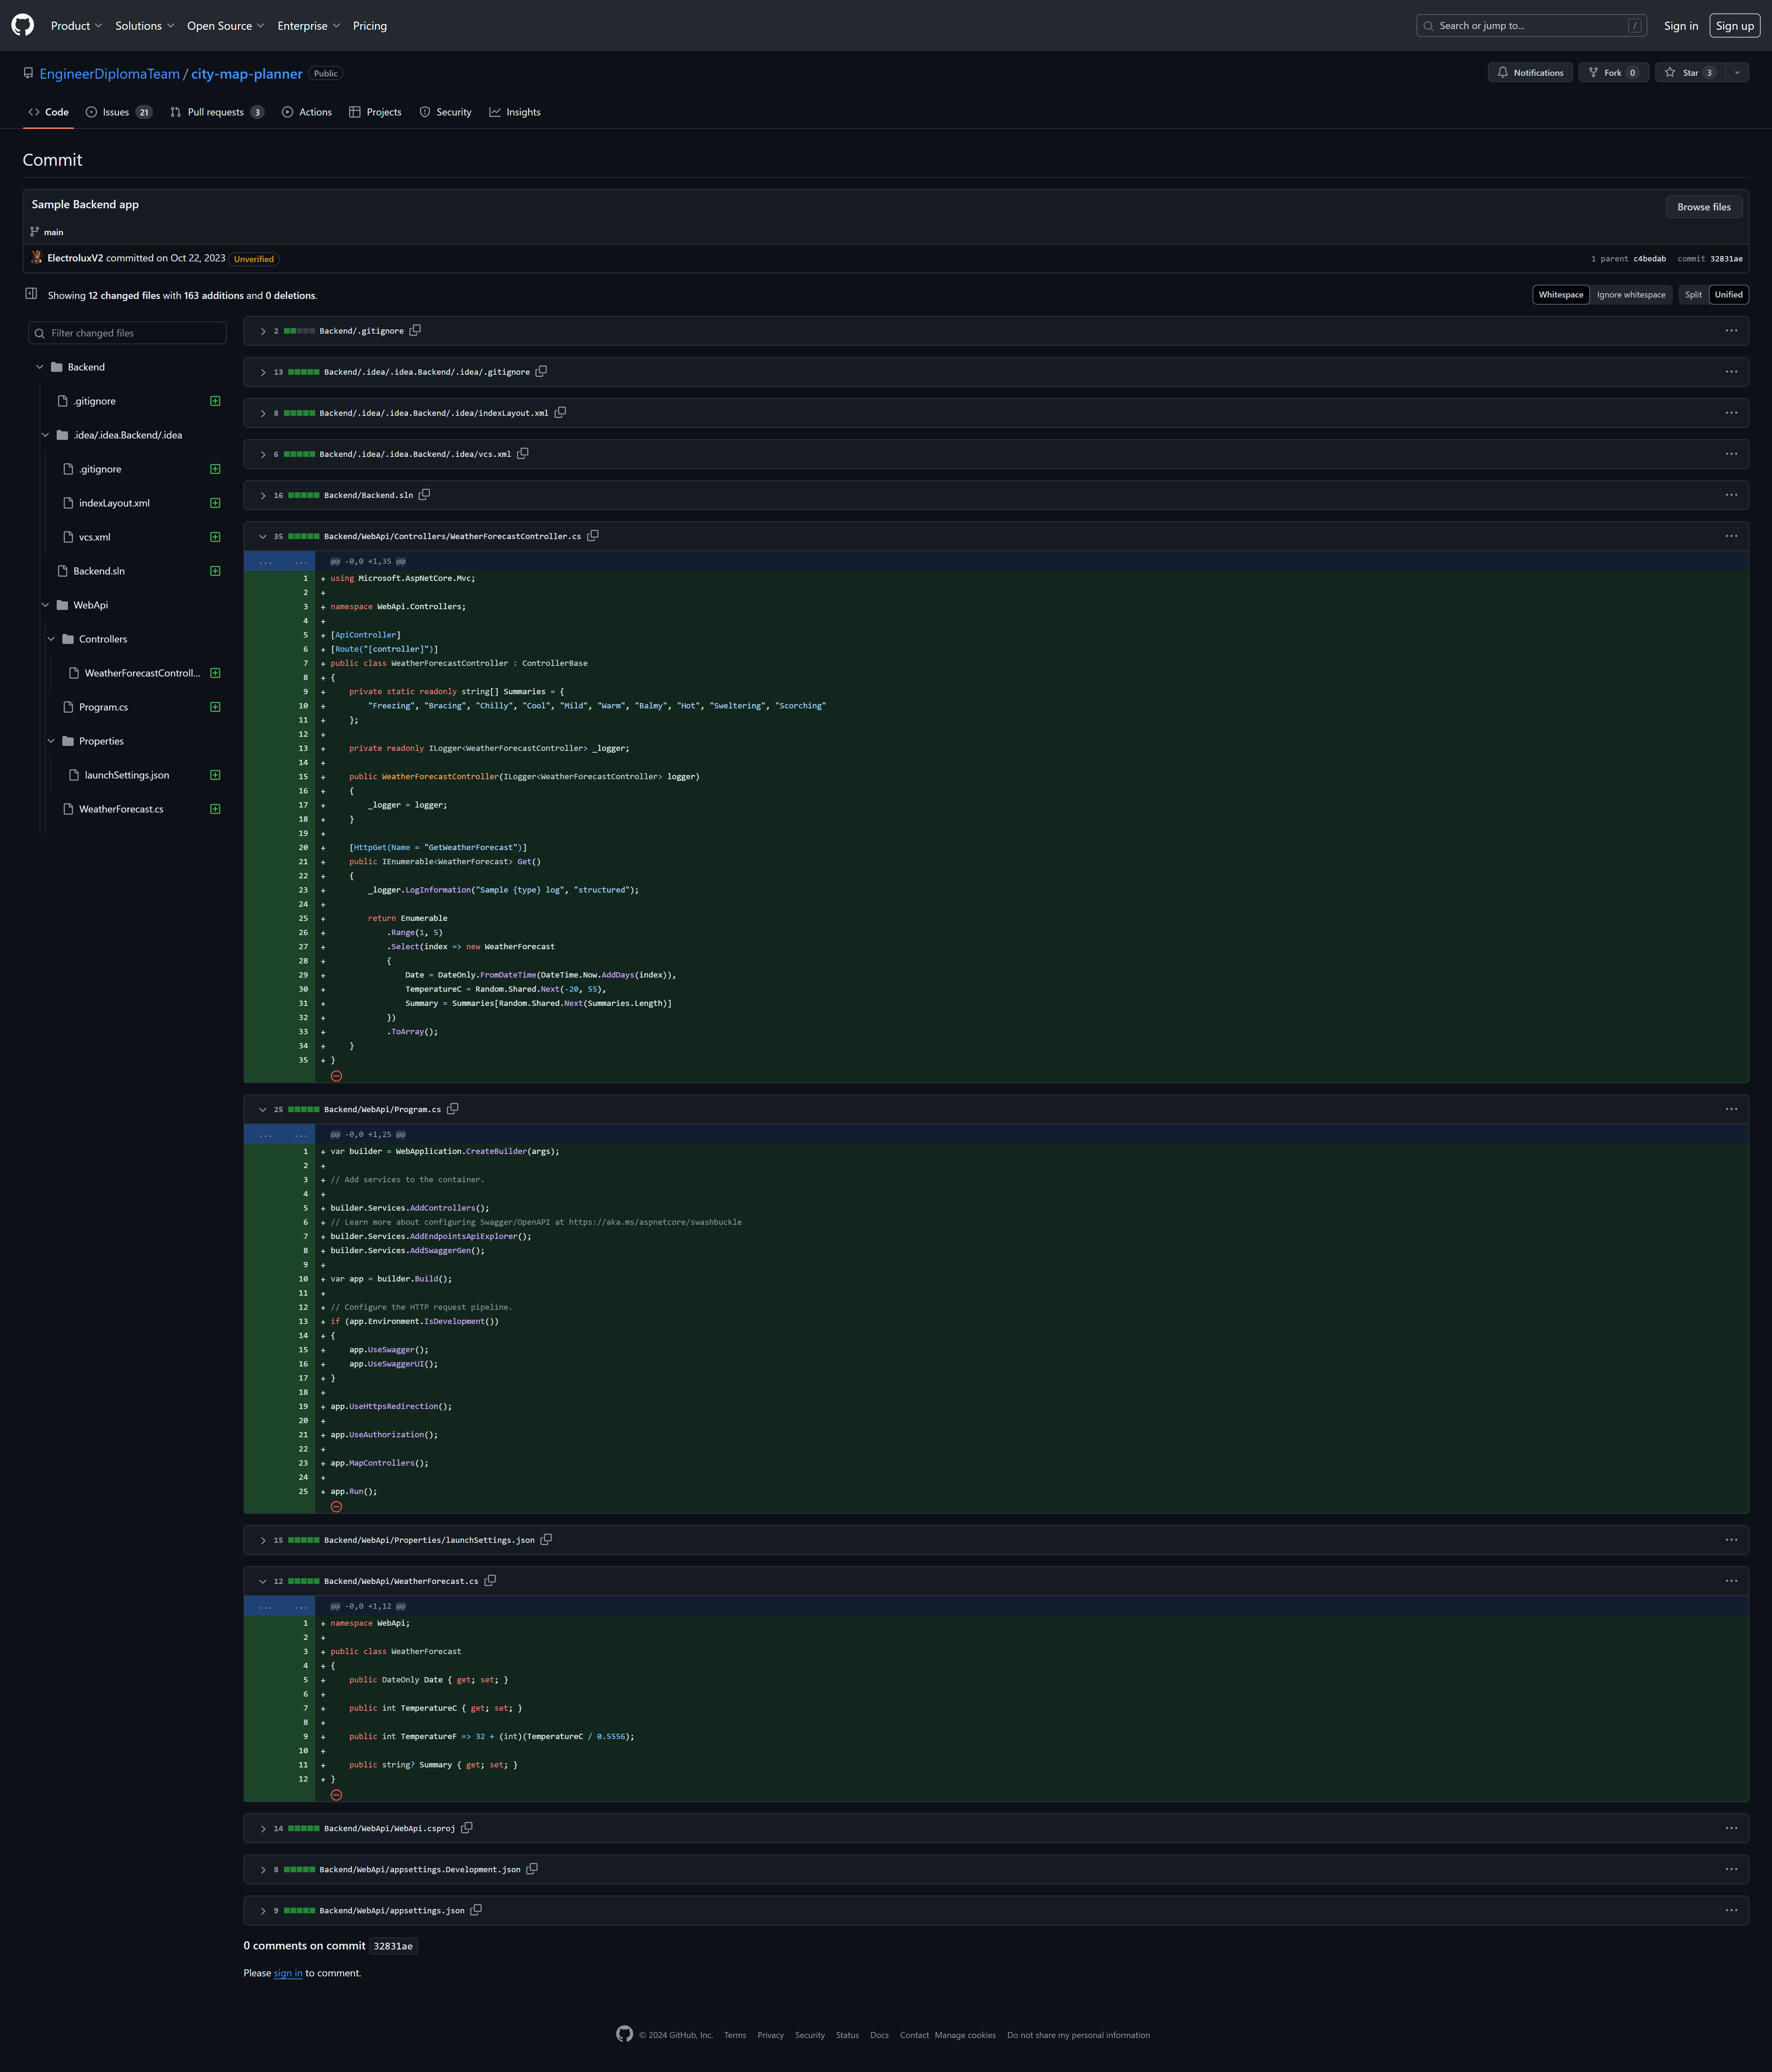
\includegraphics[width=1\textwidth]{attachments/1}
        \caption{Wykonane elementy w ramach pierwszego przyrostu}
        \label{fig:figure}
        \end{figure}
    \item frontend z ustaleniem wyglady aplikacji o oparcie Material design + api example;
    \begin{figure}[H]
        \centering
        \includegraphics[width=1\textwidth]{attachments/2}
        \caption{Wykonane elementy w ramach pierwszego przyrostu}
        \label{fig:figure}
        \end{figure}
    \item Potok ciągłego wdrożenia opisane w rozdziale 6.6;
\end{itemize}
 
Opis w czasie wykonanych zadań przestawia wykres Gantt'a
\begin{figure}[H]
    \centering
    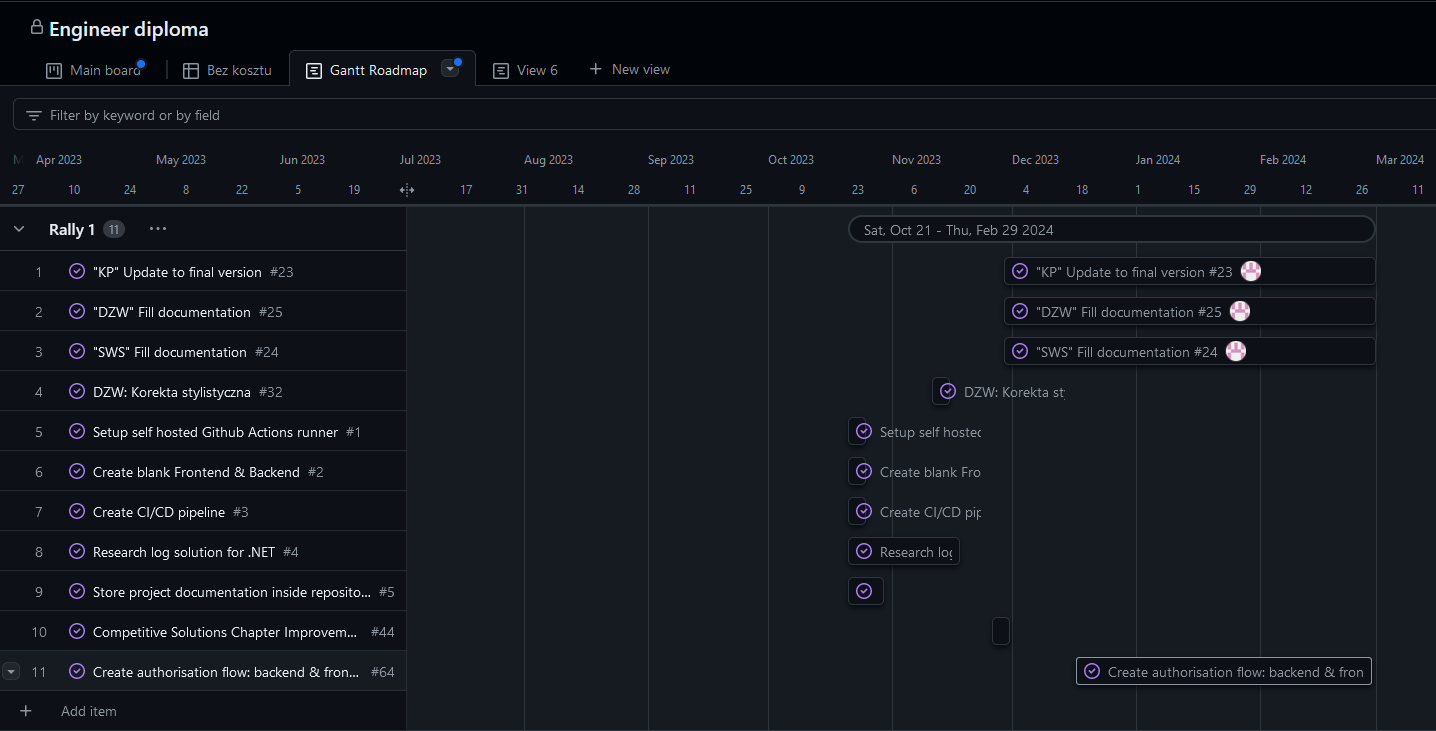
\includegraphics[width=1\textwidth]{attachments/RALLY1}
    \caption{Wykonane elementy w ramach pierwszego przyrostu}
    \label{fig:figure}
    \end{figure}

    \subsection{Przyrost II - utworzenie widoku mapy, w tym integracja  Overpass}
    \label{sec:przyrost2}

    W ramach tego przyrostu drugiego wykonano:
    \begin{itemize}
        \item OverpassAPICLIENT;
        \item Entities dla Entity Framework Core;
        \item LeaftModule;

    \end{itemize}

    https://github.com/EngineerDiplomaTeam/city-map-planner/blob/71d42c26f1de027d3ef6be6e1314b51d237d914b/Backend/WebApi.Data/Entities/BusinessTimeEntity.cs

    \subsection{Przyrost III - zarządzanie użytkownikiem}
    \label{sec:przyrost3}

    W ramach tego przyrostu trzeciego wykonano:
    \begin{itemize}
        \item widok logowania;
        \item widok rejestracji;
        \item widok zarządzania kontem;
        \item zaimplementowano autoryzacje po stronie backend;
    \end{itemize}

    https://github.com/EngineerDiplomaTeam/city-map-planner/tree/b85c21829a74f57ce20414a7fa3ab3a398ad9833/Backend/WebApi/Extensions
    https://github.com/EngineerDiplomaTeam/city-map-planner/commit/bbdbb4fdca805acd2438365551f4f361532bc34d


    \subsection{Przyrost IV - algorytm Trasy - \glslink{poidef}{POI}}
    \label{sec:przyrost4}

    W ramach tego przyrostu czwartego wykonano:
    \begin{itemize}
        \item dodanie \glslink{poidef}{POI} na mapie uzwgledniając wszystkie podstawowe informacje;
        \item dodanie algorytmu przeszukania trasy pomiędzy \glslink{poidef}{POI};
        \item dodanie ekranu koszyka z \glslink{poidef}{POI};
        https://github.com/EngineerDiplomaTeam/city-map-planner/commit/88c32b690c76b113173d056ec0be1fa74c81709a#diff-ede64cf229dabd7c007a109c15db77bcacd008a0cf42e1eacca43c3e3da9af97
        \item dodanie indywidualnych zdjeć;
        https://github.com/EngineerDiplomaTeam/city-map-planner/commit/354caede1081fe73ca98350bd1aceff95c7df8c9
        \item wykonano listę przygładowych atrakcji w Gdańsku
    \end{itemize}


    \subsection{Przyrost V - zarządzanie POI i kalendarz podróży}
    \label{sec:przyrost5}

    W ramach tego przyrostu piątego wykonano:
    \begin{itemize}
        \item integracja chatGPT;
        https://github.com/EngineerDiplomaTeam/city-map-planner/commit/989c85a11ceb0f7f9951f04838e4464c0a47d070
        \item dodanie ekranu kalendarza podróży
        \item Widok podsumowania podróży
        https://github.com/EngineerDiplomaTeam/city-map-planner/commit/796bac2b6bc5db568a7aabc7dcdef299117c2da2
        \item integracja backend oraz bazy danych z API pogodowym
        https://github.com/EngineerDiplomaTeam/city-map-planner/commit/1f899291a34701bfa61bfc0b39fd558b628bb966
        \item poprawienie widoku kalendarza
        https://github.com/EngineerDiplomaTeam/city-map-planner/commit/a3d894bcbf5c319bb2cd109a9b2c3e58db29ef56
    \end{itemize}

    \subsection{Przyrost VI - widok wszystkich atrakcji integracja pogody}
    \label{sec:przyrost5}

    W ramach tego przyrostu szóstego wykonano:
    \begin{itemize}
        \item integracja pogody widoku frontend;
        \item widok listy wszystkich POI
    \end{itemize}

